\chapter{Loss, SVM, Regularization, and Optimization Algorithms}

In a linear classifier, we have an input and a set of weights, and an output that gives some information about what class the object is in. Based on an example in the \href{http://cs231n.stanford.edu/slides/2017/cs231n_2017_lecture3.pdf}{cs231n course}, we can imagine a linear classifier that outputs class scores for every possible class. Hence, a larger number for a certain class means that it is more likely to belong to that class. Ideally, we want the value to be highest in the correct class alone.

\section{Loss Function}

We need a loss function that can help us achieve the above by expressing unhappiness with the scores across the training data. A loss function tells how good our current classifier is given a dataset of examples. The loss over the dataset is the sum of loss over examples.

\begin{equation}
    L = \frac{1}{N} \Sigma \;  L_i (f(x_i, W), y_i)
\end{equation}

Here $i$ examples, $x$ is the input features, $W$ the weights, and $y$ the ideal output while $f$ is the function we prepare. Naturally, loss should be low for correct classification and high for incorrect predictions.

\section{Support Vector Machines (SVM)}

\textit{This portion was not covered in class but is necessary to understand SVM loss - which was covered}

Stealing the following from \href{https://scikit-learn.org/stable/modules/svm.html}{scikit}:

"Support vector machines (SVMs) are a set of supervised learning methods used for classification, regression and outliers detection."

They are useful because they are effective in high dimensional spaces and effective when the number of dimensions is higher than the number of samples. It is a good method to classify with limited amount of data. 

The logic that makes SVM's work is quite interesting. It uses nonlinear data and maps the space to a higher dimension in which a linear solution exists. For instance, if our decision boundary was supposed to be a circle, we define the radius of the circle as a new dimensino $x^2 + y^2$ and can use this to classify circles of varius radii. These transformations are called \textbf{kernels}. \href{https://towardsdatascience.com/support-vector-machine-introduction-to-machine-learning-algorithms-934a444fca47}{This} has some text on what an SVM is. 

\subsection{Margins}

SVM's sound scary but as \href{https://towardsdatascience.com/support-vector-machine-simply-explained-fee28eba5496}{one person put it}, "it becomes less scary once I started to think of support vector machine as a “road machine”, which separates the left,right-side cars, buildings, pedestrians and makes the widest lane as possible. And those cars, buildings, really close to the street is the support vectors." SVM's not only want to find a decision boundary but want to maximize the margin.

Margins are the perpendicular distances between the boundary and the points close to it. Generally, we say that there is a hyper plane that classifies our data as data may not be 2 dimensional and could be of higher dimensions. In SVM's, we let the margin be $[-1, 1]$ or the classes that are formed must have been formed when the hypothesis function yielded values greater than 0 implies $y=1$ and less than 0 implies $y=-1$. Generally,

\begin{equation}
    y\cdot (\beta_0 + \beta_1 \cdot x +  \cdots + \beta_n \cdot x_n) > 0
\end{equation}

As per the previous link once again, "In the linearly separable case, SVM is trying to find the hyperplane that maximizes the margin, with the condition that both classes are classified correctly. But in reality, datasets are probably never linearly separable, so the condition of 100\% correctly classified by a hyperplane will never be met."

\subsection{Kernel Trick}

The following text is \href{https://towardsdatascience.com/support-vector-machine-simply-explained-fee28eba5496}{from the same blog above}.

"What Kernel Trick does is it utilizes existing features, applies some transformations, and creates new features. Those new features are the key for SVM to find the nonlinear decision boundary."

"Think of the polynomial kernel as a transformer/processor to generate new features by applying the polynomial combination of all the existing features."

There are various tricks and transformations that can be used to generate new features. These include polynomial kernels, radius basis kernels (uses distance between all dots to a specific dots).

Andrew NG also seems to have \href{http://cs229.stanford.edu/notes/cs229-notes3.pdf}{detailed notes on this}, but I did not read it.

\subsection{Loss}

This concept was taught with slides from \href{http://cs231n.stanford.edu/slides/2020/lecture_3.pdf}{cs231n}. 

Given an example $(x_i, y_i)$ where $x_i$ is the image and $y_i$ is the integer label.Let $f(x_i, W) = s$, the multiclass SVM loss has the form:

\begin{equation}
    l_i = \Sigma_{j \neq y_i} max(0, s_j - s_{y_i} + 1)
\end{equation}

Here $s_j$ is the score for the class j and $s_{y_i}$ is the real class of the example. This is similar to RELU which is an activation function. We will look at this later. It is generally of the form $f(x) = max(0, x)$. This is also called hinge loss.

\textbf{Interesting Problem: Look at question 7 of the slides}

\section{Regularization}

Imagine that we have a set of points, and we want to create a function to model this data. Now, we can have a very simple function that approximates the points, or a very high dimension one that fits all of training data. The latter cause will usually result in overfitting and may perform poorly for the test data. 

Regularization can be done in many ways but the common way to do it involves adding a term to Loss:

\begin{equation}
    L = \frac{1}{N} \Sigma \;  L_i (f(x_i, W), y_i) + \lambda R(W)
\end{equation}

There are various forms of regularization:

\begin{itemize}
    \item L2: We assume that the weights are a matrix and we sum the squares of all the elements. This likes to "spread out" the weights.
    \item L1: We sum the absolute values of the matrix. This makes the weight matrix sparse - only few non-zero weights.
    \item Elastic Net: It is like the sum of L2 and L1 regularization with a parameter for L2.
    \item More complex: Dropout and Batch normalization. Will be covered later.
\end{itemize}

Regularization helps make the model simpler - occam's razor. 

\subsection{Batch Normalization}

\begin{equation}
    \hat{x} = \frac{x-E[x]}{\sqrt{Var[x]}}
\end{equation}

This forces a gaussian distribution for the inputs-- at the end of every fully connected layers. We can also normalize with mini batch mean and variance. So this would ensure that we don't have a predictable gaussian input. The unit gaussian isn't always the best though because sometimes we want some saturation and choosing a normalization that allows for this gives the network room to learn what's required. 

\subsection{Dropout}

Let's assume that we have a network which can classify well - with it's set of neurons. Some neurons can be imagined to look for certain features (a nose, a tail, etc). With dropout, we remove some of these neurons (squash them to zero) and try getting the model to perform well with this set of neurons. A different subset of units is randomly selected every time we present a training example. Hence, we are able to prevent co-adaptation (presence of all features). The absence of certain features should let us generalize well. This helps prevent overfitting basically.

Look at random forest - start out with a large set of neurons and prune the set as some become unnecessary.

\subsection{Data Augmentation}

This involves modifying existing some images in certain ways - change the orientation, dimensions, or "augment" it. We then train the data on this. We can have a random set of crops/scales as well, shear, and much more.

\subsection{DropConnect}

In drop connect, we drop certain connections (set some weights to zero) instead of the nodes, so they can remain partially active. DropConnect is a generalization of DropOut because it produces even more possible models, since there are almost always more connections than units. However, you can get similar outcomes on an individual trial. 

\subsection{Mixup}

In mixup, we train on random blends of images (blend the pixels of various images for instance). This has been found to improve generalization. Google for more details.

\subsection{Transfer Learning}

We always need a lot of data to train a neural network. We can do this without data augmentation using "Transfer Learning". As the name suggests, you ‘transfer’ the weights the network learns and learn some more with the small dataset. That is, you fine tune the network for the new dataset, keeping the weights of the previous one. The myth that we need a large dataset is hence broken for training networks. This makes sense for similar data as a result where fine tuning is more benefitial than training from scratch. This is called 'restore model' since we are restoring the state from a previously trained network and continuing from there. 

\section{Softmax Classifier (Multinomial Logistic Regression)}

Let us assume that we have a vector $s$ of real numbers. The softmax function will take this vector as an input and assign probability scores to each of the element as follows:

\begin{equation}
    \sigma(s)_k = \frac{e^{s_k}}{\sum_j e^{s_j}}
\end{equation}

Now when applied, this will give us a column vector with probabilities for each class. Now, to get the loss for the example $i$ is:

\begin{equation}
    L_i = -\log P(Y=y_i | X=x_i) \text{where $y_i$ is the correct classification}
\end{equation}

Clearly Softmax function is extremely useful for classification problems. One question that may come up is "Why use softmax instead of normalizing the values derived?". As per \href{http://93.174.95.29/main/11874B3F9B89BAB4C7826272B2EFC032}{section 2.3.3 of Deep Learning by the "godfathers of AI"}, having exponentiated variables help since we tend to calculate the log likelihood.

This is also called cross-entropy loss. Since, this error is given as a probability, it's easier to visualize the error with Softmax. Unlike SVM, where we cannot infer any such thing.

\section{Stochastic Gradient Descent}

Gradient descent is computationally inefficient when the dataset is very large as for every update step, we need to calculate average loss across all examples. Additionally, the drop in loss may not be much to begin with. Hence, we can use "minibatches" as sample of the training data for gradient descent. This sample can be arbitrary and not fixed. Hence, this will perform better. In online stochastic gradient descent, size of minibatch is 1.

The problem with stochastic gradient descent is that it is more sensitive to only certain weights. Hence, it's making very slow progress to reach the global minima as the progress along a certain dimension due to a lack of sensitivity in one dimension. This is possible since we are using mini-batches and noise may easily get into our data.

Problems also exist with local minima and with flat surfaces as the global minima cannot be reached. 

\section{Other Optimization Methods}

Gradient descent was an algorithm that helped us explore our search space. It is also called an optimzation algorithm. They essentially serve the purpose of minimizing our loss function. Gradient descent isn't the only such method! Few more optimization methods are discussed in the 'Optimization' chapter in the SLAM section. While the ones in this section may focus on variations of SGD, they tend to focus on second order approximations (kinda). The concepts are one and the same - getting a quicker, better convergence.

\subsection{SGD + Momentum}

This is something that will commonly be used. In a regular SGD, we use the regular update equation as stochastic gradient descent. In SGD+Momentum, we also calculate velocity and rather than moving in the direction of negative gradient, we move in direction of velocity. The idea is that even at a local minima, the "ball" stuck at the local minima will have momentum and velocity. Now, if we have a local minima it will likely be a small hill and using this momentum we can escape the local minima. Even at saddle points (flatish surfaces), there is some velocity as well and hence we can move from this position. 

We don't just go in direction of velocity but with the weighted sum of velocity and gradient.

If SGD was \[ x_{t+1} = x_t - \alpha \nabla f(x_t) \]

Now, in SGD + Momentum:

\begin{equation}
\begin{split}
    v_{t+1} = \rho v_t - \alpha \nabla f(x_t) \\
    x_{t+1} = x_t + v_{t+1}
\end{split}
\end{equation}

From cs231n notes:

As an unfortunate misnomer, this variable $\rho$ is in optimization referred to as momentum (its typical value is about 0.9), but its physical meaning is more consistent with the coefficient of friction. Effectively, this variable damps the velocity and reduces the kinetic energy of the system, or otherwise the particle would never come to a stop at the bottom of a hill. 

\subsection{AdaGrad}

AdaGrad keeps a runnning sum estimate of the squared gradients. So instead of velocity, we have a "gradient squared" term. The update equation is essentially:

\begin{equation}
\begin{split}
    x_{t+1} = x_t - \alpha \frac{\nabla f(x_t)}{\sum_t (\nabla f(x_t))^T + 1e^{-7}} \text{ where 1e-7 is to prevent 0 division }
\end{split}
\end{equation}

\textbf{Why does this help?}

If our gradient is high, then the square of the gradient will be higher. If gradient is low, then dividing by this makes the update more sensitive to a lower sensitvity variable. In AdaGrad, progress along ‘steep’ directions is damped and progress along ‘flat’ directions is accelerated. But over time, the step size gets smaller and smaller. It’s good in the convex case because as you approach the minima, you want to slow down and converge. But in non convex case, if you come across a saddle point, you get stuck and can’t make any progress.

\subsection{RMSProp}

The problem with AdaGrad is that the sum of gradient squares will become very big constantly. And, in the end we'll be taking very tiny steps towards minima. RMSProp solves this. It is a leaky AdaGrad. Here, we'll just let the sum of gradient squares \textbf{decay} over time as can be seen in figure \ref{fig:rms+prop}.

\begin{figure}[h]
    \centering
    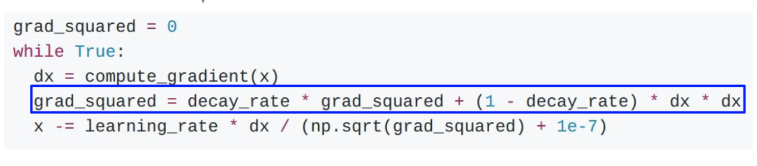
\includegraphics[width=12cm]{img/RMSProp.png}
    \caption{RMS Prop Calculation}
    \label{fig:rms+prop}
\end{figure}
\subsection{Adam}

The core idea behind momentum is to move in the direction of velocity to not get stuck in a local minima. The core idea behind AdaGrad was to compute the square of the gradients to slow down movement along the sensitive direction and prevent zig-zags. The core idea behind Adam is to combine the two! This can be seen in \ref{fig:adam}.

\begin{figure}[h]
    \centering
    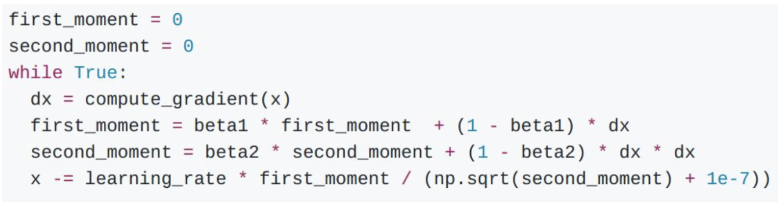
\includegraphics[width=12cm]{img/adam.png}
    \caption{Adam Calculation}
    \label{fig:adam}
\end{figure}

The problem with Adam is that at the first step the second moment is 0. Hence, when divided by such a small near 0 quantity, the value of $x$ will change significantly. This is a problem with RMSProp/AdaGrad as well. Of course, since the first moment is also very small, it may cancel out the second moment, but sometimes, it does result in taking very large steps in the beginning. This is solved with a bias correction step.

\href{https://youtu.be/_JB0AO7QxSA?t=2588}{cs231n} covers these quite well.

Adam is the best algorithm and converges really quick. Abhinav vouches for it. His recommendations for setting up Adam are:

\begin{enumerate}
    \item beta1 = 0.9
    \item beta2 = 0.999
    \item learning\_rate = 1e-3 or 5e-4
\end{enumerate}

\subsection{Misc: Learning Rate $\alpha$}

It is the number by which we multiply the resulting gradient by. The size of the steps that we take across iterations are defined by learning rate. Generally, as the loss value reduces, we lower the learning rate - slow down as we are nearly about to converge. SGD, SGD+Momentum, AdaGrad, RMSProp, and Adam all have learning rate as a hyperparameter.

‘Step Decay’ - we reduce the learning rate at particular steps, so if it would’ve gotten stuck somewhere, we can take smaller baby steps and maybe reach a better region. 

\section{Data Processing}

Before training the model, it is important that our input data meets certain standards and model isn't regularized. We've already seen how regularization helps generalize the model. Another way of ensuring this is to modify the input data with data preprocessing.

We can imagine that the input data has high variance and is off center (not near origin). Hence, we can zero-center the data - subtract mean of data from each element of the dataset. We can then divide the dataset by the standard deviation of the datasetand normalize the dataset. This helps prevent gradient extinguishing and gradient explosions. 